\renewcommand{\theequation}{\theenumi}
\begin{enumerate}[label=\thesection.\arabic*.,ref=\thesection.\theenumi]
\numberwithin{equation}{enumi}
\item The histogram of given data set is represented in fig. \ref{fig:Q44}
\begin{figure}[!ht]
\centering
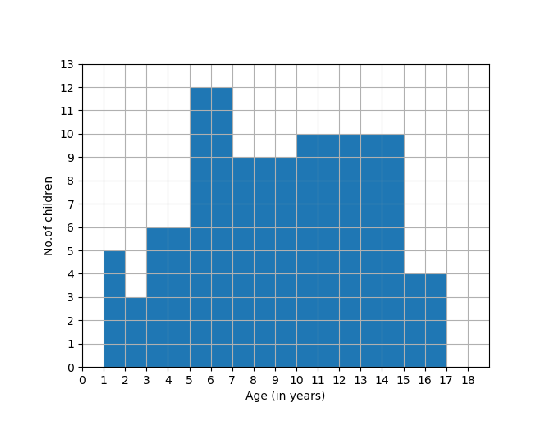
\includegraphics[width= \columnwidth]{./statistics/figs/Q44.eps}
\caption{Histogram showing No.of children vs. age(in years)}
\label{fig:Q44}
\end{figure}
\item The python code for the plot can be downloaded from
\begin{lstlisting}
statistics/codes/Q44.py
\end{lstlisting}

\end{enumerate}